\documentclass[tikz,border=2pt]{standalone}
\usepackage{amsmath}
\usetikzlibrary{arrows.meta,calc}
\begin{document}
% B = P^{-1}AP as a commuting square: going up with P, across with A and down with P^{-1} equals
% going across with B. Example: A = [[4,1],[2,3]], P = [[1,1],[1,-2]], B = diag(5,2); same eigenvalues.
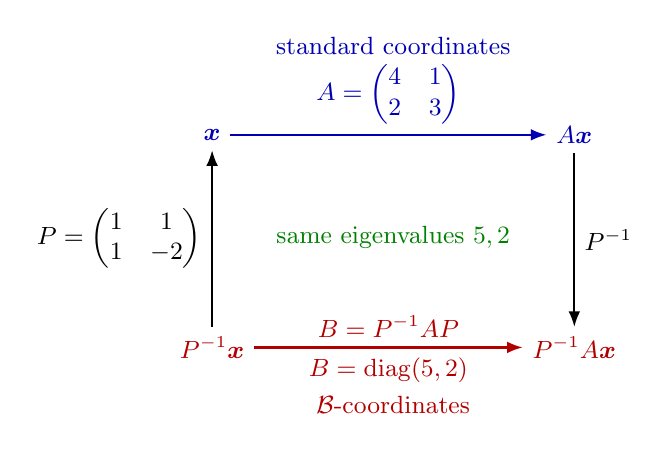
\begin{tikzpicture}[font=\small, >={Latex[length=2mm]}]
  \node[blue!70!black] (x)  at (0,2.7) {$\boldsymbol{x}$};
  \node[blue!70!black] (Ax) at (4.6,2.7) {$A\boldsymbol{x}$};
  \node[red!70!black]  (y)  at (0,0) {$P^{-1}\boldsymbol{x}$};
  \node[red!70!black]  (By) at (4.6,0) {$P^{-1}A\boldsymbol{x}$};
  \draw[->, thick, blue!70!black] (x) -- (Ax)
    node[midway, above] {$A=\begin{pmatrix}4&1\\2&3\end{pmatrix}$};
  \draw[->, thick, red!70!black] (y) -- (By)
    node[midway, above] {$B=P^{-1}AP$}
    node[midway, below] {$B=\operatorname{diag}(5,2)$};
  \draw[->, thick] (y) -- (x) node[midway, left] {$P=\begin{pmatrix}1&1\\1&-2\end{pmatrix}$};
  \draw[->, thick] (Ax) -- (By) node[midway, right] {$P^{-1}$};
  \node[blue!70!black, anchor=south] at ([yshift=9mm]$(x)!0.5!(Ax)$) {standard coordinates};
  \node[red!70!black, anchor=north] at ([yshift=-5mm]$(y)!0.5!(By)$) {$\mathcal{B}$-coordinates};
  \node[green!50!black, anchor=center, align=center] at (2.3,1.4) {same eigenvalues $5,2$};
\end{tikzpicture}
\end{document}
